\section{Aspectos Claves en la Gestión y Dirección del Conocimiento}

De cuando en cuando en el mundo científico aparecen nuevas perspectivas acerca de como abordar algunos de los problemas con los que la humanidad ha lidiado y así obtener las soluciones más efectivas y eficientes que los minimicen, y quizás, los erradiquen. Lo anterior nunca ocurre sin un costo siendo uno de los primeros el de la concertación aceptada por la comunidad del término que describe el nuevo paradigma. Es lógico que un solo nombre no puede englobar toda la descripción del paradigma y, a partir de esta concepción reduccionista, pueden surgir desacuerdos agnósticos por parte de aquellos que no comprenden la  completa extensión del modelo.

En la gestión del conocimiento ocurre que varios autores \cite{firestone2001}, \cite{bergeron2003}, \cite{davenport1998}; entre muchos otros, pretenden erróneamente consolidar una única definición “perspectivística “ de la propuesta sin considerarla a partir de una visión sistémica que lo transcienda a lo que en investigación holística se comprende como sintagma\cite{hurtado2000}. La \textit{gestión de conocimiento}, como se percibe en la presente investigación, es “una unión sintagmática de diversos paradigmas” \cite{hurtado2000}, estos se distinguen de acuerdo a sus componentes claves  algunos de los cuales, quizás los más relevantes al objeto mismo de la investigación, son revisados a continuación.

\subsection{Acerca del conocimiento}

En la presente investigación conocimiento es entendido como un concepto que encierra, entre otras, las siguientes definiciones y se usarán de acuerdo a su contexto como partes complementarias de una misma meta – definición.

Partiendo de la definición clásica compilada por Gunter Dueck\cite{dueck2001}, el conocimiento es un concepto que puede tener componentes en una o varias de las siguientes dimensiones:

\begin{itemize}
\item  \textbf{Episteme} -\textit{ Dimensión abstracta – o metafísica}, en forma de generalizaciones, bases, leyes y principios científicos.

\item \textbf{Phronesis }– \textit{Dimensión práctica}, relativa al conocimiento pragmático discernido a través de las practicas aceptadas por la sociedad.

\item \textbf{Techne} – \textit{Dimensión técnica}, relativa a la forma de hacer las cosas, de la realización de actividades concretada en la forma de manuales, procedimientos y comunidades de práctica.

\item \textbf{Metis} – \textit{Dimensión objetiva}, como forma de volver corpóreo, real y sustancial la conjugación de los otros tipos de conocimiento.
\end{itemize}

Es esta concepción multidimensional la que justifica completamente la investigación acerca de sistemas informáticos que soporten las tareas de estructuración de conocimiento integral. Definiciones posteriores extienden y explican más claramente la taxonomía del conocimiento dada por los griegos:

“El conocimiento incluye restricciones implícitas y explícitas entre objetos (entidades), operaciones y relaciones, que permiten recoger heurísticas generales y específicas así como los procedimientos de inferencias relacionados con la situación a modelar”.\cite{sowa1984}

“El conocimiento es información organizada y analizada para hacerla comprensible y aplicable a la resolución de problemas y toma de decisiones”.\cite{turban1992}

“El conocimiento se compone de verdades y creencias, perspectivas y conceptos, juicios y expectativas, metodologías y know-how”.\cite{wiig1993}

“Creencia justificada que incrementa la capacidad de una entidad para la acción efectiva”. Lo que le adiciona un valor subjetivo al conocimiento según \cite{nokata1994}

\subsection{Ciclo de Conocimiento}

Múltiples factores deben ser considerados cuando se trata de capturar, crear y diseminar el conocimiento dentro de un grupo de personas. La no homogeneidad en los medios de almacenamiento de conocimiento es uno de ellos. El conocimiento - en cualquiera de sus formas, puede estar guardado en diferentes partes que van desde entidades biológicas - mente humana, genes; a repositorios de conocimiento estructurado tales como ontologías, grafos de relación o mapas mentales.

Otro factor importante es la capacidad de acceso al conocimiento que es muy diferente al mero hecho de acceder a una fuente de conocimiento dada. En \cite{nokata1995} se considera que el conocimiento puede estar en dos estadios con propiedades diferentes: tácito y explícito. 

\begin{itemize}
\item \textbf{Conocimiento tácito:} Este conocimiento se corresponde con el conocimiento obtenido a través de la experiencia, conocimiento simultáneo  y conocimiento análogo. Esta forma de conocimiento usualmente se encuentra en medios de almacenamiento biológicos como la mente humana.

\item \textbf{Conocimiento explícito:} Se corresponde con el conocimiento racional, conocimiento secuencial, y conocimiento digital y se encuentra almacenado en documentos, bases de conocimiento, ontologías o cualquier otro medio abstracto de representación.
\end{itemize}

En \cite{liebowitz1998} se establece un tercer estadio llamado conocimiento implícito.

\begin{itemize}
\item \textit{Conocimiento Implícito:} Acceso directo mediante consulta y discusión. Requiere la localización y comunicación previa de conocimiento informal.
\end{itemize}

Un \textit{Ciclo de Conocimiento} es el proceso por el cual el conocimiento se transforma de tácito a explícito y viceversa por medio de las siguientes actividades:

\begin{itemize}
\item \textbf{Socialización:} Compartir conocimiento tácito entre individuos. El conocimiento permanece siendo tácito sin ser transformado en explícito. Este tipo de patrón no es muy interesante debido a su naturaleza tácita (Tácito - Tácito).

\item \textbf{Articulación:} Alguien transforma el conocimiento tácito en explícito (Tácito - Explícito).

\item \textbf{Síntesis:} Combinación de conocimiento explícito para crear nuevo conocimiento explícito  (Explícito - Explícito).
 
\item \textbf{Interiorización:} Proceso de transformar conocimiento explícito en tácito (Explícito - Tácito).
\end{itemize}

\begin{figure}
 \centering
 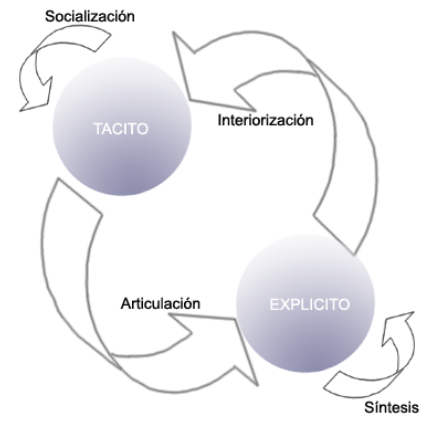
\includegraphics[width=156mm, height=156mm]{Ciclo_Conocimiento.png}
 \caption{Ciclo de Conocimiento}
 \label{ciclo_conocimiento}
\end{figure}

El flujo de conocimiento organizacional más importante es la transformación del conocimiento tácito en explícito \cite{wiig1993}, esto es, la \textit{articulación} que se apoya en procesos avanzados de socialización. Esto permite acumular conocimiento explícito que puede ser compartido y accedido por los miembros de la organización. Por el contrario, la interiorización es el proceso natural llevado a cabo a través del aprendizaje individual por parte de los integrantes de la organización, esto es, la asimilación de conocimiento. 

El tercer flujo de conocimiento relacionado con la transformación de conocimiento es la \textit{combinación} o síntesis. En este caso se transfiere conocimiento a otra forma explícita de conocimiento. Un ejemplo sería el cambiar el formato de una base de conocimiento, agrupar ontologías o refinar heurísticas. Este tipo de flujo de conocimiento es importante para seleccionar, combinar y distribuir el conocimiento existente con diferentes fines. Por ser quizás el flujo de conocimiento más formal en el SITEM algunos componentes específicos implementan flujos de síntesis de conocimiento.

El cuarto flujo del ciclo de vida del conocimiento permite transformar conocimiento tácito en otras formas de conocimiento tácito mediante procesos de socialización. Un ejemplo de esto es cuando se transfiere conocimiento tácito de un experto a un ingeniero de conocimiento en una entrevista personal.

\subsection{Tecnologías del Conocimiento}

En la actualidad el conocimiento se considera un activo fundamental y como lo expresan \cite{martinez1998}, tiene dos propiedades de vital importancia para contribuir al desarrollo de las organizaciones o comunidades de práctica:

\begin{itemize}
\item \textbf{Es explicable.} Cuando no se evidencia esta propiedad el conocimiento permanece tácito y en ninguna medida puede considerarse como perteneciente a la comunidad o la organización. Es entonces una tésis que solo aquel conocimiento que se ha convertido en explícito es el que posee una organización; de otra manera es propiedad exclusiva del individuo.

\item \textbf{Se puede comunicar y compartir.} Cuando no se toman medidas que formalicen estas actividades el conocimiento se pierde. Es decir, la organización o comunidad debe tener procesos conocidos que garanticen flujos de conocimiento basados en la síntesis, interiorización y socialización.
\end{itemize}

En general para que el conocimiento pueda generar ventajas competitivas debe ser gestionado de alguna manera. Esta necesidad dio surgimiento a dos áreas de investigacion comunmente agrupadas bajo el concepto de Tecnologías de Conocimento: Ingeniería de Conocimiento y Gestión de Conocimiento. 

Uno de los primeros problemas que deben atacar las tecnologías de conocimiento es el asociado con el Modelado de Conocimiento. En \cite{wielinga1992} se expresan algunos principios a tener en cuenta cuando se modela el conocimiento:

\begin{itemize}
\item \textbf{Definición de roles de conocimiento}. El conocimiento se puede dividir en unidades atómicas que tienen propiedades irreductibles y que se asocian para lograr funciones que identifican dicha unidad.

\item \textbf{Identificación de tipos de conocimiento.} Cada unidad de conocimiento debe enmarcarse en uno o varios de los siguientes tipos de conocimiento: de tareas, inferencial, del dominio, ontologías del dominio, modelos del dominio. 

\item \textbf{Capacidad de ser compartido y reutilizado.} Las unidades de conocimiento pueden ser expresadas usando lenguajes y reglas formales. Lo que permite que pueda ser entendido por entidades con roles de conocimiento definidos.

\item \textbf{Uso de modelos gráficos.} La unidades de conocimiento pueden ser representadas mediante grafos tipo red en los cuales tanto los nodos como las rutas de interconexión son unidades atómicas de conocimiento.
\end{itemize}


\subsection{Gestión de conocimiento}

Fue \textit{Karl Wiig}, quien usó el término de \textit{gestión de conocimiento} por primera vez durante una conferencia en Suiza y a partir de ese momento diversos autores han conceptualizado el término surgiendo definiciones parciales tales como:

“La Gestión de Conocimiento es la construcción y aplicación sistemática, explícita y deliberada de conocimiento para maximizar la efectividad organizacional con respecto al conocimiento, por lo que usa sus activos de conocimiento”\cite{wiig1993}

“La Gestión de Conocimiento es el proceso de capturar experiencia colectiva organizacional donde ésta resida (por ejemplo, bases de datos, documentos, mentes humanas) y su distribución allá donde pueda ayudar a mejorar los resultados”\cite{hibbard1997}

“La Gestión de Conocimiento es la gestión y control explícito del conocimiento en una organización para lograr los objetivos de la organización” (van der Spek and Spijkervet, 1997)

Consecuente con la concepción de la gestión de conocimiento como un sintagma se puede concebir un paradigma asociado a un proceso con ciertas actividades implicadas: (Dignum y Heimannsfeld, 1999) 

\begin{itemize}
\item Identificación y mapeo de bienes intelectuales de la organización.
\item Generación de conocimiento nuevo que permita obtener una ventaja competitiva. 
\item Recopilación accesible de información organizacional. 
\item Compartir buenas prácticas y tecnología, incluyendo técnicas de trabajo en grupo.
\end{itemize}

Este paradigma explora el conocimiento técnico, pragmático y objetivo considerando que la conjugación de leyes rígida e epistemológicas van en contravía de la dinámica misma de los sistemas. La articulación de este conocimiento debe ser mantenido de alguna forma en la organización, y de ahí surge el concepto de Memoria Corporativa. El saber hacer está completamente diseminado en la organización y debe ser integrado de forma coherente para facilitar el acceso al mismo y su reutilización, esto es, expresarlo en forma de memoria corporativa. 

Las memorias corporativas se consideran un elemento clave para gestionar el conocimiento porque facilitan su conservación, distribución y reutilización. Van Heijst define la memoria corporativa como una “representación de conocimiento e información organizacional explícita y persistente”, mientras que en (Nagenda y Plaza, 1996) se define como “los recursos colectivos de datos y conocimiento de una compañía, incluyendo experiencias en proyectos, experiencia en resolución de problemas, etc”. En (Abecker, 1998), una memoria corporativa es referida como “un contenedor que integra información contextual, documentos e información no estructurada, que facilita su uso y reutilización”.

%\section {Ontologias}


1.5 ONTOLOGÍAS

Tal como ocurre con el conocimiento, el concepto de ontología ha recibido múltiples definiciones a lo largo de la historia y es necesario aclarar que, una vez más y debido a sus múltiples usos, el término trasciende sus raíces etimológicas y filosóficas para convertirse en si mismo en un concepto con semántica de tipo contextual. Inicialmente para la filosofía una ontología es una 
“Parte de la metafísica que trata del ser en general y de sus propiedades trascendentales.” Diccionario de la Real Academia de la Lengua

“Ciencia o estudio del ser: específicamente, una rama de la metafísica relacionada con la naturaleza y las relaciones del ser; un sistema particular según el cual se investigan los problemas de la naturaleza del ser; esto es, filosofía fundamental”.

“Teoría relativa a los tipos de entidades y específicamente los tipos de entidades abstractas que se admiten en el lenguaje de un sistema” 

Q!ueda claro que el término ha sido tomado prestado de ls escuales filosóficas y es por ende allí en donde se puede obtener un contexto más apropiado que pèrmita concretar lo que, en el campo de la gestión de conocimiento, una ontología pretende englobar.

La “Oxford Companion of Philosophy” define ontología de la siguiente forma: 

 “Ontología, entendida como una rama de la metafísica, es la ciencia del ser en general,       abarcando aspectos como la naturaleza de la existencia y la estructura categórica de la       realidad. El término ontología tiene algunos usos adicionales en filosofía. En un sentido       derivativo se usa para referirse a un conjunto de cosas cuya existencia queda reconocida por una teoría o sistema de pensamiento. En este sentido se habla de la ontología de una teoría o de un sistema metafísico definido por tal ontología”

Y es por esto que la ontología puede ser concebida como una forma de reconocer – formalizar, la existencia de supuestos metafísicos tales como el conocimiento. Es esta formulación la que comúnmente es aceptada en el área de la inteligencia artificial sobre todo la expresada por Quine (Quine, 1961), quien dijo que todo lo que puede ser cuantificado existe.

La primera definición de ontología en Inteligencia Artificial apareció en (Neches et al, 1991):

“Una ontología define los términos básicos y relaciones que conforman el vocabulario de un área específica, así como las reglas para combinar dichos términos y las  relaciones para definir extensiones de vocabularios”

Una de las definiciones más extendidas es la dada por Tom Gruber (Gruber, 1993): 

 "Una ontología es una especificación explícita de una conceptualización. El término       proviene de la filosofía, donde una ontología es un recuento sistemático de la existencia. En sistemas de Inteligencia Artificial, lo que existe es lo que puede ser representado. Cuando el conocimiento de un dominio se representa mediante un formalismo declarativo, el conjunto de objetos que puede ser representado se llama universo del discurso. Esos conjuntos de objetos, y las relaciones que se establecen entre ellos, son reflejados en un vocabulario con el cual representamos el conocimiento en un sistema basado en conocimiento. Así, en el contexto de IA, podemos describir la ontología de un programa como un conjunto de términos. En tal ontología, las definiciones asocian nombres de entidades del universo del discurso con textos comprensibles por los humanos que describen el significado de los nombres, y axiomas formales que limitan la interpretación y buen uso de dichos términos. Formalmente, una ontología es una teoría lógica”
     
Gruber entiende por conceptualización “una interpretación estructurada de una parte del mundo que usan los seres humanos para pensar y comunicar sobre ella. Para un informático, una conceptualización podría ser la clasificación de sistemas informáticos atendiendo a su naturaleza física en sistemas hardware, sistemas software y sistemas firmware.” (Fernández, 2003). Además dicha conceptualización debe ser, de alguna forma, factible de ser compartida y entendida.

Nicola Guarino (Guarino, 1995) tratando de crear una definición concertada  expresó:

“Un punto de inicio en este esfuerzo clarificador será el cuidadoso análisis de la       interpretación dada por Gruber. El problema principal de dicha interpretación es que se basa en la noción de conceptualización. Una conceptualización es un conjunto de relaciones extensionales que describen un estado particular, mientras que la noción que tenemos en mente es intensional, esto es, algo como una rejilla conceptual al que le imponemos varios posibles estados ...En el sentido filosófico, podemos referirnos a una ontología como un sistema particular de categorías que representa una cierta visión del mundo. Como tal, este sistema no        depende de un lenguaje particular: la ontología de Aristóteles es siempre la misma,       independientemente del lenguaje usado para describirla. Por otro lado, en su uso más típico en IA, una ontología es un artefacto ingenieril constituido por un vocabulario específico para describir una cierta realidad, más un conjunto de supuestos explícitos concernientes al significado pretendido de las palabras del vocabulario. Este conjunto de supuestos tiene generalmente la forma de teorías lógicas de primer orden, donde las palabras del vocabulario aparecen como predicados unarios o binarios, respectivamente llamados conceptos y relaciones. En el caso más simple, una ontología describe una jerarquía de conceptos relacionados por relaciones de subsunción; en los casos más sofisticados, se añaden axiomas para expresar otras relaciones entre conceptos y restringir la posible interpretación.”

Más tarde Guarino modificaría su definición para abarcar conceptos más globales para la interpretación afirmando que: 

“Una ontología puede especificar una conceptualización en una forma muy indirecta, puesto que i) solo puede aproximar un conjunto de modelos pretendidos; y ii) tal conjunto de modelos pretendidos sólo es una caracterización débil de una conceptualización.”. (Guarino, 1998)

Borst (Borst, 1997), redefine la ontología de Gruber:

“Una ontología es una especificación formal de una conceptualización compartida.” 

A la par que (Studer et al, 1998) explica que:
“Conceptualización se refiere a un modelo abstracto de algún fenómeno en el mundo a través de la identificación de los conceptos relevantes de dicho fenómeno. Explícita significa que el tipo de conceptos y restricciones usados se definen explícitamente. Formal representa el hecho de que la ontología debería ser entendible por las máquinas. Compartida refleja la noción de que una ontología captura conocimiento consensual, esto es, que no es de un individuo, sino que es aceptado por un grupo” 

Con lo anterior se puede tener una visión adecuada de las ontologías – quizás no completa pero práctica, que permite asociar técnicas a la definición propia de estructuras que modelen y sirvan para expresar – socializar, el estado de conceptos abstractos.

1.5.1 Tipos de ontologías
      
En general las ontologías, referidas como medio para modelar sistemas abstractos, pueden ser clasificadas de acuerdo a ciertos criterios como son: (a) el tipo de conocimiento contenido; y (b) la motivación de la ontología.

1.5.1.1. Ontologías según el conocimiento contenido

Este es el criterio donde existe mayor diversidad, la cual puede ser ilustrada por las dos siguientes clasificaciones de ontologías. La primera de ellas fue propuesta en (Van Heijst et al, 1997), donde se distinguen tres tipos de ontologías: 
Ontologías terminológicas, lingüísticas: Especifican los términos usados para representar conocimiento en el dominio. Un ejemplo de este tipo de ontologías es la red semántica UMLS (Unified Medical Language System) (Lindberg et al, 1993).

Ontologías de información: Especifican la estructura de los registros de la base de datos. Los esquemas de bases de datos serían un ejemplo. 

Ontologías para modelar conocimiento: Especifican conceptualizaciones de conocimiento. Estas ontologías tienen una estructura interna mucho más rica que los anteriores tipos de ontologías, y éstas son las ontologías que interesan a los desarrolladores de sistemas basados en conocimiento.      

Una clasificación alternativa fue propuesta en (Mizoguchi et al, 1995), donde también se proponen tres categorías:

Ontologías del dominio: Contienen todos los conceptos asociados a un dominio particular.
Ontologías de tarea: Establecen la forma en la cual se puede usar el conocimiento del dominio para realizar tareas específicas. De esta forma, una aplicación podría realizar búsquedas de información mientras otra podría gestionar la asignación de bloques libre de memoria.
Ontologías generales: Contienen descripciones generales sobre objetos, eventos, relaciones    temporales,   relaciones    causales, modelos de  comportamiento y funcionalidades.

1.5.1.2. Ontologías por motivación para su creación

Inicialmente se distinguen cuatro tipos de ontologías:

Ontologías para la representación de conocimiento: Permiten explicar las conceptualizaciones que subyacen de los formalismos de representación de conocimiento (Davis et al, 1993).

Ontologías genéricas: Definen conceptos considerados genéricos en diferentes áreas. Ejemplos de tales conceptos serían componente, subclase, proceso, estado, etc. Estas ontologías son reutilizables en diferentes dominios. Se llaman también ontologías abstractas o superteorías porque permiten definir conceptos abstractos, y dichas ontologías pueden ser usadas para definir conceptos de forma más específica en diferentes dominios. Como ejemplos podemos ver la taxonomía, la mereología, la topología y la teoría general de sistemas.

Ontologías del dominio: Definen conceptualizaciones específicas del dominio. Las metodologías actuales de adquisición de conocimiento distinguen entre ontologías y conocimiento del dominio, porque el último describe situaciones factuales del dominio, mientras que las ontologías imponen descripciones sobre la estructura y contenido del conocimiento del dominio.

Ontologías de aplicación: Están ligadas al desarrollo de una aplicación concreta. Tales ontologías cubren los aspectos relacionados con aplicaciones particulares. Típicamente, estas ontologías toman conceptos de ontologías del dominio y genéricas, así como métodos específicos para realizar la tarea, por lo que no son muy adecuadas para ser reutilizadas.

Una clasificación alternativa fue propuesta por Poli (Poli, 2000). En dicha clasificación se identifican los siguientes tipos de ontologías: 

Ontologías generales: Tienen que ver con las categorías fundamentales y sus conexiones de dependencia. Con respecto a las categorías fundamentales, los investigadores se dan cada vez más cuenta de la dificultad de manejar este nivel supremo. Por ello, es de máxima importancia emplear una organización de categorías principales que sea lo más transparente posible. Existen categorías fundamentales que se aplican a todos los niveles ontológicos. Sin embargo, muchas de las categorías top- level pueden tener diferentes valores en niveles diferentes de la ontología, aunque deben  tener algo en común. 

Ontologías categóricas: Estudian las diversas formas en las que una categoría se da cuenta de los diversos niveles ontológicos, determinando la posible presencia de una teoría general que subsume sus concretizaciones. Mientras que la ontología general está más relacionada con la arquitectura de la teoría, la ontología categórica es más sensible a los detalles de las categorías individuales. Sin embargo, es obvio que ambas son necesarias.

Ontologías del dominio: Se refieren a la estructuración detallada de un contexto de análisis con respecto a los subdominios que lo componen. 

Ontologías genéricas: Parecen ligadas a corpus lingüísticos y léxicos conceptuales. De hecho, se pueden clasificar los términos en varios niveles. Esto significa que cada término debería ser accesible por defecto únicamente en su sentido genérico, mientas que sus significados especializados quedan para cuando se active una ontología del dominio específica. Por otro lado, la ontología del dominio contiene términos que no tienen correspondencias analíticas en ontologías genéricas. El conocimiento del dominio “satura” el conocimiento genérico.

Ontología regional: Analiza las categorías y sus conexiones de interdependencia para cada nivel ontológico (estrato o capa). 

Ontología aplicada: Estas ontologías son la aplicación concreta de entorno ontológico a un objeto específico (por ejemplo, un proyecto).

 1.5.2. Ontologías de tipo Formal y Descriptiva

Una tercera clasificación se basa en el grado de formalidad de la ontología. Según este criterio se distinguen tres tipos de ontologías en (Poli, 2002): 

Ontología descriptiva, relacionada con la recolección de información sobre los ítems del dominio analizado. La unidad y variedad del mundo es la salida de las conexiones de dependencia y formas de independencia entre los ítems. Cosas materiales, plantas y animales, así como los productos de los talentos y actividades de animales y humanos, son ítems del mundo. 

En otras palabras, el mundo no solo contiene cosas, animadas o no, sino también actividades y procesos, así como los productos derivados de los mismos. Es difícil negar que existen pensamientos, sensaciones y decisiones, así como el completo espectro de actividades mentales, así como uno está obligado a admitir la existencia de reglas, lenguajes, sociedades y costumbres (Poli,2001a).        

Ontología formal, que destila, filtra, codifica y organiza los resultados de una ontología descriptiva. Según esta interpretación, la ontología formal es formal en el sentido usado por Husserl es sus “Logical Investigations”. Ser formal en este sentido implica tratar con categorías como cosa, proceso, materia, forma, todo, parte, etc. Estas categorías caracterizan aspectos y tipos de realidad que todavía no han sido utilizados bajo ningún formalismo.        

La codificación formal en sentido estricto se da al nivel de ontología formalizada. El objetivo es encontrar la codificación formal apropiada para los constructores adquiridos de forma descriptiva y purificarlos formalmente como se indica. El nivel de construcciones formalizadas también está relacionado con la evaluación de la adecuación (expresiva, computacional, cognitiva) de los distintos formalismos, y con el problema de las traducciones recíprocas. La fuerte similaridad entre los términos “formal” y “formalizada” es un contratiempo. Una forma de evitar la confusión es utilizar “categórica” en vez de formal. La mayor parte de las teorías contemporáneas sólo reconocen dos niveles de análisis y suelen unir las categorías formales con el análisis formalizado. Como consecuencia, se suele negar la relevancia específica de los análisis categóricos. 

Los tres niveles ontológicos son diferentes pero no están separados, puesto que están relacionados en muchos aspectos. El conocimiento descriptivo puede referirse a categorías formales, y las salidas formalizadas a los otros dos niveles. Por otro lado, es más delicado establecer las diferencias y conexiones entre varias facetas ontológicas como se muestra en (Poli, 2002a).        

La aplicación de métodos lógico-formales a una ontología la transforma en ontología formal. Los primeros ontólogos formales creían que la tarea de construcción podía ser llevada a cabo de forma sistemática y está completamente basada en la resolución de problemas lógicos, esto es, en la gramática lógica de lenguajes particulares. En contraste, la antigua tradición ontológica se ha quedado en un almacén de intuiciones ontológicas, constituyendo argumentos informales e incluso retóricos sobre esas intuiciones como base. Como se establece en (Gangemi et al, 1999),       las relaciones formales implican entidades de todas las esferas materiales, de forma que son comprensibles per se como nociones universales. Por el contrario, las relaciones materiales son específicas de una o más esferas materiales. Esto presupone una división a priori del dominio en esferas materiales: primero se debe realizar una distinción entre relaciones formales y materiales con base a su comportamiento con respecto a tales subdominios. De esta forma, las relaciones formales establecen las conexiones y las diferencias entre subdominios primitivos, mientras que las relaciones materiales caracterizan las propiedades de un subdominio específico. Si se asume un dominio plano, sin estructura a priori, entonces no sería válida la distinción entre relaciones formales y materiales. 

1.5.3 Ingeniería Ontológica

Las ontologías proporcionan un vocabulario común de un área y definen, a diferentes niveles de formalismo, el significado de los términos y relaciones entre ellos. El conocimiento en ontologías se formaliza principalmente usando cinco tipos de componentes: clases, relaciones, funciones, axiomas e instancias (Gruber, 93).

Las clases en la ontología se suelen organizar en taxonomías. Algunas veces, la noción de ontología se diluye en el sentido que las taxonomías se consideran ontologías completas [Studer et al.; 98]. Se suele usar tanto el término clases como conceptos. Un concepto puede ser algo sobre lo que se dice algo y, por lo tanto, también podría ser la descripción de una tarea, función, acción, estrategia, proceso de razonamiento, etc. 

Las relaciones representan un tipo de interacción entre los conceptos del dominio. Se definen formalmente como cualquier subconjunto de un producto de n conjuntos, esto es: 
R: C1 x C2 x ... x Cn.
Como ejemplos de relaciones binarios incluimos: “subclase de” y “conectado a”. Las funciones son un tipo especial de relaciones en las que el n-ésimo elemento de la relación es único para los n-1 precedentes. Formalmente, definimos las funciones F como: 
F: C1 x C2 x ... x Cn-1 x  Cn. 
Como ejemplos podemos mencionar las funciones “madre de” y “precio de un coche usado”. 

Los axiomas son expresiones que son siempre ciertas. Pueden ser incluidas en una ontología con muchos propósitos, tales como definir el significado de los componentes ontológicos, definir restricciones complejas sobre los valores de los atributos, argumentos de relaciones, etc verificando la corrección de la información especificada en la ontología o deduciendo nueva información. Tales ontologías son llamadas ontologías pesadas, en contraste con las ontologías ligeras que no incluyen axiomas. 

Las instancias se usan para representar elementos específicos.

1.5.3.1. Relaciones

En (Gómez-Pérez et al, 2000) se enumeran las relaciones más comunes en dominios reales, a saber: equivalencia, taxonómica, partonómica, dependencia, topológica, causal, funcional, cronológica, similaridad, condicional y propósito. Sin embargo, no todas las relaciones tienen la misma relevancia ni imponen el mismo tipo de propiedades jerárquicas a la ontología. Entre este conjunto de relaciones podemos subrayar tres de ellas: taxonomía, mereología, y topología. Taxonomía.

La palabra taxonomía tiene su origen en dos términos griegos, a saber, taxis (orden) y nomos (tratado) y esta palabra proviene de la Filosofía. Taxonomía es la ciencia que estudia la división en grupos ordenados o categorías. Desde un punto de vista ontológico, una taxonomía es una organización ontológica basada en una relación de orden parcial llamada IS-A, a través de la cual se agrupan las entidades y son subsumidas por clases de más ato nivel. En general, las taxonomías han sido importantes para modelar esquemas de bases de datos, sistemas basadas en
conocimiento y vocabularios semánticos (Guarino and Welty, 2001).

A continuación se presentan las propiedades satisfechas por las relaciones taxonómicas. Con este propósito, se usará la notación empleada en (Guarino and Welty, 2001). De esta forma, se dice que un individuo x perteneciente a una clase OJO::::

Asimetría: Esta propiedad significa que la inclusión de una clase de individuos, X, en una clase Y implica la no inclusión de Y en X. Formalmente, esta propiedad garantiza que: (X es a Y) si y solo si no ocurre que (Y es a X).

Transitividad: Sea X incluido en una clase Y, que a su vez está incluido en una clase Z, ambas inclusiones a través de relaciones.

Irreflexividad: Admitir la reflexividad en relaciones taxonómicas solo tendría sentido para modelar tautologías. Una tautología es la expresión de un mismo hecho de distintas maneras. La relación taxonómica se considera no reflexiva.

Existen otras propiedades taxonómicas que están relacionadas con los atributos de los conceptos a través de la taxonomía:

Redefinición: Esta propiedad consiste en cambiar el nombre de una propiedad común a dos conceptos, padre e hijo, y se asigna un nombre diferente al atributo en el hijo. 

Herencia múltiple: Esta propiedad está asociada con atributos conceptuales. Un concepto puede tener diferentes padres taxonómicos, así que este concepto heredaría propiedades de todos sus padres. 

Además de las propiedades taxonómicas básicas, existen otras condiciones basadas en cuestiones filosóficas relacionadas con taxonomías. Algunas de estas condiciones se señalan en (Guarino and Welty, 2001):

Identidad
Unidad
Esencia
Dependencia
Rigidez

Las dos primeras condiciones se enlazan al concepto filosófico de “ser”. Según Guarino, las intuiciones tras ambos conceptos requieren, con la finalidad de comprenderlos, hacer una distinción entre ellos. Así, la condición de identidad se relaciona al problema de distinguir una instancia de su clase específica de instancias de la misma clase, por medio de lo que llamamos “propiedad característica”, la cual es única para cada instancia.


\subsubsection{Sistemas de Gestión de Conocimiento}

En IA, las bases de conocimiento son generadas para ser consumidas en sistemas expertos y basados en conocimiento, donde las computadoras usan inferencias para responder a cuestiones de usuario. Aunque es importante la adquisición de conocimiento para inferencias computacionales, en los desarrollos más recientes en Gestión del Conocimiento, el conocimiento queda disponible para consumo humano directo o para desarrollar software que procese dicho conocimiento. 

Históricamente, la Gestión de Conocimiento se ha centrado en un único grupo a través de lo que generalmente se ha conocido como sistema de información ejecutiva (EIS), que contiene un conjunto de herramientas para acceder a bases de datos, generar alertas, etc para apoyar el proceso de toma de decisiones. Más recientemente, se ha comenzado a diseñar sistemas de Gestión de Conocimiento para organizaciones completas. Si los ejecutivos necesitan acceder a la información y al conocimiento, es probable que sus empleados tengan interés en esa información.
 
De acuerdo con (O´Leary, 1999) citado por (Valencia, 2005), las principales funciones de un sistema de gestión de conocimiento son facilitar:

\begin{itemize}
\item La conversión de datos y texto en conocimiento;
\item La conversión de conocimiento individual y de grupo en conocimiento explícito;
\item La conexión de individuos y conocimiento a otros individuos y conocimientos;
\item La comunicación de información entre diferentes grupos;
\item La creación de nuevo conocimiento útil para la organización;
\end{itemize}

\subsubsection{Sistemas Integrados para el Soporte de Desempeño}

Sistemas que integran múltiples fuentes y herramientas de gestión de conocimiento en un único ambiente de trabajo para apoyar de una manera más efectiva las tareas relacionadas con: (Winslow and Bramer, 1994)

\begin{itemize}
\item \textbf{Infraestructura:} Organización y estructura del entorno de trabajo. 
\item \textbf{Control:} Monitorización, coordinación y control.
\item \textbf{Navegación:} Interacción hombre-máquina.
\item \textbf{Presentación:} Posibilidad para personalizar datos y servicios.
\item \textbf{Adquisición:} Captura conocimiento, casos, opiniones, aprendizaje y datos sensoriales en diferentes medios y su transformación en formato interno.
\item \textbf{Consultoría:} Consultar servicios, asistencia y recordatorios.
\item \textbf{Instrucción:} Ayuda y entrenamiento.
\item \textbf{Aprendizaje:} Aplicación de técnicas de descubrimiento de conocimiento y minería de datos.
\item \textbf{Evaluación:} Valoración y certificación basada en medidas del rendimiento y la calidad.
\item \textbf{Referencia:} Constituyen fuentes de conocimiento y experiencia para la organización.
\end{itemize}

Estos sistemas se han convertido en la actualidad en una necesidad debido al crecimiento desmesurado de aplicaciones incompatibles y protocolos no estandarizados. 